%---------------------------------------------------------------------------------------------------------------------------
\section{Résolution graphique d'(in)équations} 
%---------------------------------------------------------------------------------------------------------------------------

\subsection{Lecture graphique des images et des antécédents}

\begin{multicols}{2}

    Nous considérons la fonction
    \begin{equation}
        \begin{aligned}
            f\colon \eR&\to \eR \\
            x&\mapsto x^2 
        \end{aligned}
    \end{equation}
    dont le graphe est donné ci-contre. À chaque réel $x$, nous associons l'abscisse $y=f(x)$.  À l'aide du graphe donné, répondre aux questions suivantes.

    \begin{itemize}
        \item Image de $1,5$ ? 
        \item Antécédent de $3,5$ ?  
        \item Antécédent de $-1$ ? 
        \item Antécédent de $0$ ? 
    \end{itemize}

    \columnbreak

    %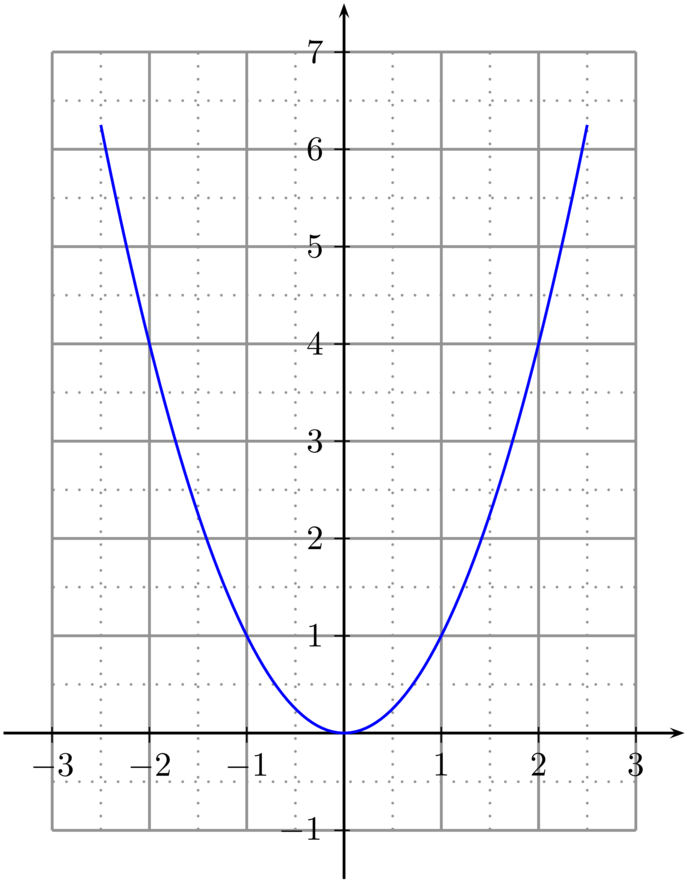
\includegraphics{Picture_FIGLabelFigFCarreQFhsWzPICTFCarreQFhsWz-for_eps.pdf}
    %\newcommand{\CaptionFigFCarreQFhsWz}{Le graphe de la fonction \( x\mapsto x^2\).}
    \input{Fig_FCarreQFhsWz.pstricks}

\end{multicols}

  \begin{example}
Compléter le tableau suivant pour la fonction $f(x)=x^2$.
\begin{equation}
\begin{array}[h]{|c|c|c|c|c|c|c|c|c|c|c|c|}
  \hline  
  x & -4 & -3 & -2 & -1 & 0 & 1 & 2 & 3 & 4 & -0,5 & 0,5  \\
  \hline
  y & 16 &&&&&&&&&&0.25\\
  \hline
\end{array}
\end{equation}
  \end{example}


\subsection{Résolution graphique d'équations}

\begin{Aretenir}
    Soit $k$, un réel fixé. Résoudre l'équation $f(x)=k$ revient à chercher les antécédents par $f$ du nombre $k$.

Le nombre de solutions de l'équation $f(x)=k$ est égal au nombre de points d'intersection de la courbe représentative de \( f\) avec la droite $d$ d'équation $y=k$. Les solutions sont les abscisses de ces points d'intersection. 
\end{Aretenir}


\begin{example}
    \begin{multicols}{2}
  Nous cherchons à résoudre $f(x)=4$. 
  \begin{itemize}
      \item 
          Nous traçons la droite horizontale d'équation \( y=4\);
      \item
          nous observons les points d'intersection de cette droite avec la courbe;
      \item
          les solutions de l'équation sont les abscisses de ces points.
  \end{itemize}

\columnbreak


%The result is on figure \ref{LabelFigExCarrexvfvre}. % From file ExCarrexvfvre
%\newcommand{\CaptionFigExCarrexvfvre}{<+Type your caption here+>}
\input{Fig_ExCarrexvfvre.pstricks}

    \end{multicols}

    Sans surprises, les solutions de \( x^2=4\) sont \( x=2\) et \( x=-2\).

\end{example}

\begin{Aretenir}
    Résoudre l'équation $f(x)=g(x)$ revient à déterminer les abscisses des points d'intersection des courbes représentatives de \( f\) et \( g\).
\end{Aretenir}


\begin{multicols}{2}

    Les solutions de l'équation \( f(x)=g(x)\) sont les abscisses des points d'intersection des deux courbes. Pour les trouver, il suffit de repérer les points d'intersections, puis de les projeter sur l'axe horizontal.

    Dans le cas de la figure ci-contre, les solutions sont approximativement \( x=-3.6\), \( x=-1.1\) et \( x=1.5\).

\columnbreak

%The result is on figure \ref{LabelFigExEquationIntersectioniSHPTw}. % From file ExEquationIntersectioniSHPTw
%\newcommand{\CaptionFigExEquationIntersectioniSHPTw}{<+Type your caption here+>}
\input{Fig_ExEquationIntersectioniSHPTw.pstricks}

\end{multicols}


\subsection{Résolution graphique d'inéquations}


%///////////////////////////////////////////////////////////////////////////////////////////////////////////////////////////
\subsubsection{Inéquation du type $f(x)<k$}
%///////////////////////////////////////////////////////////////////////////////////////////////////////////////////////////

\begin{Aretenir}
Les solutions de l'inéquation $f(x)<k$ sont les abscisses des points de $\mathscr{C}$ situés en-dessous de la droite d'équation $y=k$.

En particulier, les solutions de l'inéquation $f(x)<0$ sont les abscisses des points de la courbe représentative de \( f\) situés en-dessous de l'axe des abscisses, c'est-à-dire ayant une ordonnée strictement négative.
\end{Aretenir}

\begin{multicols}{2}
    Sur la figure ci-contre, nous résolvons \( f(x)\leq 2\). La procédure à suivre est la suivante.
    \begin{enumerate}
        \item
            Tracer la droite horizontale \( y=2\).
        \item
            Trouver les points d'intersection avec le graphe de \( f\).
        \item
            Les solutions sont les abscisses pour lesquelles le graphe de \( f\) est au-dessus du graphe de la droite \( y=2\).
    \end{enumerate}

    \columnbreak

%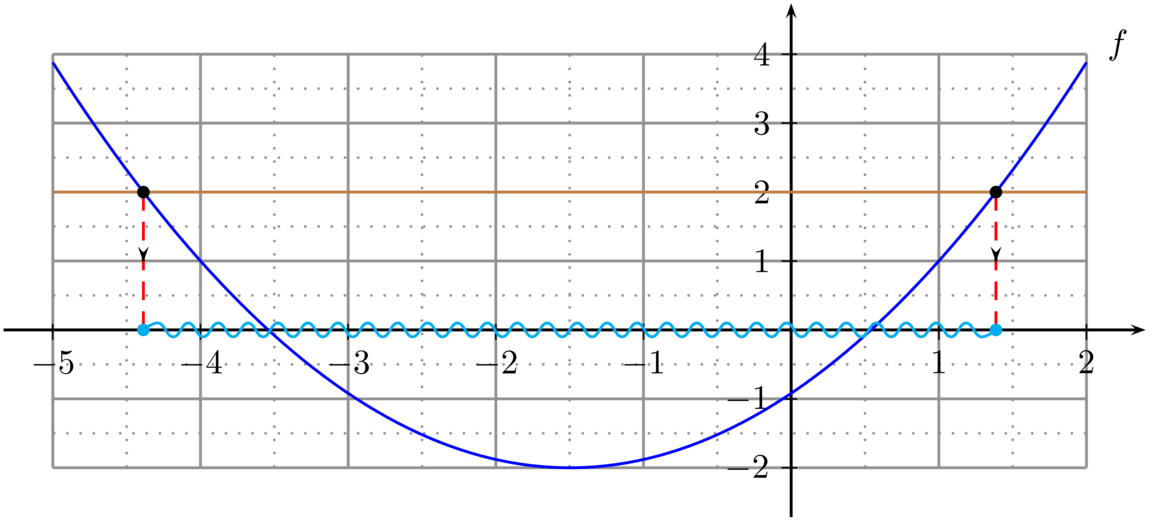
\includegraphics{Picture_FIGLabelFigExIneqOcAWMqPICTExIneqOcAWMq-for_eps.pdf}
    %\newcommand{\CaptionFigExIneqOcAWMq}{Les solutions de l'équation \( f(x)\leq 2\) sont en ondulé.}
    \input{Fig_ExIneqOcAWMq.pstricks}

\end{multicols}


\begin{remark}
    Ici nous avons résolut l'équation \( f(x)\leq 2\). Les deux points extrêmes dont partie de l'ensemble des solutions. Si nous avions résolu \( f(x)<2\), alors les points extrêmes n'auraient pas fait partie de l'ensemble des solutions.
\end{remark}

On procède de la même manière pour les inégalités du type $f(x)>k$, $f(x)\geq k$, $f(x)\leq k$. 

%///////////////////////////////////////////////////////////////////////////////////////////////////////////////////////////
\subsubsection{Inéquation du type $f(x)<g(x)$}
%///////////////////////////////////////////////////////////////////////////////////////////////////////////////////////////

Les solutions de l'inéquation $f(x)<g(x)$ sont les abscisses des points pour lesquels la courbe de \( f\) est en-dessous de la courbe de \( g\).


\newcommand{\CaptionFigExIneqfgZWStde}{En cyan, l'ensemble des solutions de l'inéquation \( f(x)<g(x)\).}
\input{Fig_ExIneqfgZWStde.pstricks}

La figure \ref{LabelFigExIneqfgZWStde} montre la résolution d'une telle inéquation. Notons que l'ensemble des solutions peut être en plusieurs morceaux.


\section{Sens de variation d'une fonction}

\subsection{Notion intuitive}

\begin{multicols}{2}

    La fonction ci-contre descend jusqu'à \( -2.5\) puis monte entre \( -2.5\) et \( 2\) pour ensuite descendre.

    Nous disons qu'elle est
    \begin{itemize}
        \item 
            \emph{décroissante} sur \( \mathopen] \infty , -2.5 \mathclose]\);
        \item
            \emph{croissante} sur \( \mathopen[ -2.5 , 2 \mathclose]\);
        \item
            à nouveau décroissante sur \( \mathopen[ 2 , \infty [\).
    \end{itemize}
    
    \columnbreak

%    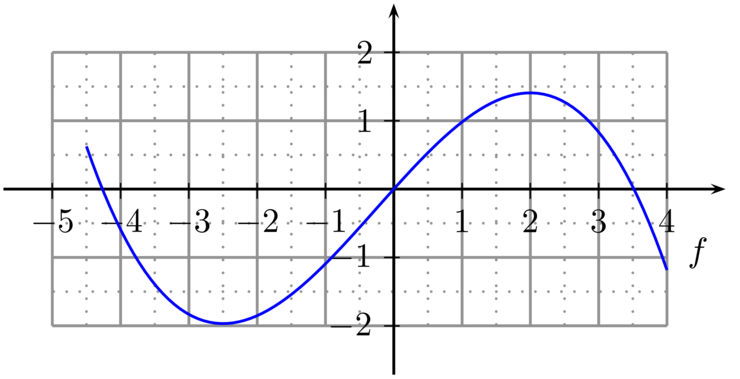
\includegraphics{Picture_FIGLabelFigExVariationRXTkocPICTExVariationRXTkoc-for_eps.pdf}
%The result is on figure \ref{LabelFigExVariationRXTkoc}.
%\newcommand{\CaptionFigExVariationRXTkoc}{<+Type your caption here+>}
\input{Fig_ExVariationRXTkoc.pstricks}

\end{multicols}


\subsection{Définition}

\begin{definition}
      Soit $f$ une fonction définie sur $\defD$ et $I$ un
      intervalle de $\defD$.\\[-2ex]
      \begin{enumerate}
          \item On dit que $f$ est \defe{croissante}{croissante (fonction)} sur $I$
        si et seulement si pour tous réels $a$ et $b$ de $I$, 
        si $a\leq b$ \ alors \ $f(a)\leq f(b)$.
    \item On dit que $f$ est \defe{décroissante}{décroissante (fonction)} sur $I$
        si et seulement si pour tous réels $a$ et $b$ de $I$, 
        si $a\leq b$ \ alors \ $f(a)\geq f(b)$. 
      \end{enumerate}
\end{definition}


\begin{remark}
    Une fonction croissante range les images dans le même ordre que les antécédents. Une fonction décroissante inverse cet ordre. 
\end{remark}


\begin{definition}
    On dit que $f$ est \defe{strictement croissante}{strictement croissante} sur~$I$
  si pour tous réels $a$ et $b$ de $I$ tels que $a<b$, on a $f(a)<f(b)$.

  La fonction \( f\) est \defe{strictement décroissante}{strictement décroissante} sur \( I\) si pour tous réels $a$ et $b$ de $I$ tels que $a<b$, on a $f(a)>f(b)$.
\end{definition}
La différence entre la croissance et la \emph{stricte} croissance est que l'inégalité est stricte.

\begin{definition}
    Soit \( I\) un intervalle de \( \eR\). Nous disons que la fonction \( f\) est \defe{monotone}{monotone} sur $I$ si elle est soit croissante sur $I$, soit décroissante sur $I$.
\end{definition}

\begin{multicols}{2}

    La fonction dessinée ci-contre n'est pas monotone sur l'intervalle \( \mathopen[ -2 , 0 \mathclose]\). Elle est
    \begin{itemize}
        \item 
            monotone décroissante sur \( \mathopen[ -2.5 , -1 \mathclose]\);
        \item
            monotone croissante sur \( \mathopen[ -1 , 1 \mathclose]\);
        \item
            monotone décroissante sur \( \mathopen[ 1 , 1.5 \mathclose]\).
    \end{itemize}

\columnbreak

%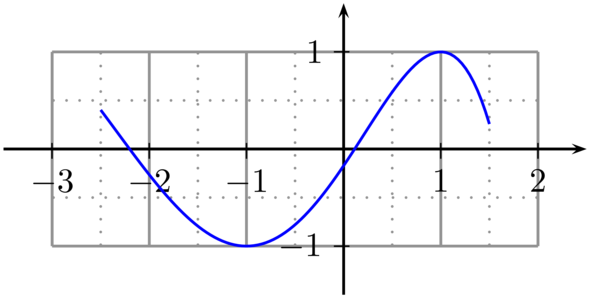
\includegraphics{Picture_FIGLabelFigGrapheVarndvdQMPICTGrapheVarndvdQM-for_eps.pdf}
%The result is on figure \ref{LabelFigGrapheVarndvdQM}.
%\newcommand{\CaptionFigGrapheVarndvdQM}{<+Type your caption here+>}
\input{Fig_GrapheVarndvdQM.pstricks}

\end{multicols}




\begin{definition}
    Soit \( I\) un intervalle. On dit que $f$ est \defe{constante}{constante (fonction)} sur $I$ lorsque pour tous les réels $a$ et $b$ de $I$, on a $f(a)=f(b)$. (Tous les réels de $I$ ont la même image par $f$).
\end{definition}

\begin{multicols}{2}
    Dans ce cas, il existe $k\in\eR$ tel que pour tout $a\in I$, $f(a)=k$. 
    
    La figure ci-contre donne le graphe de la fonction \( f(x)=1.5\) entre \( x=-3\) et \( x=3\).

\columnbreak

%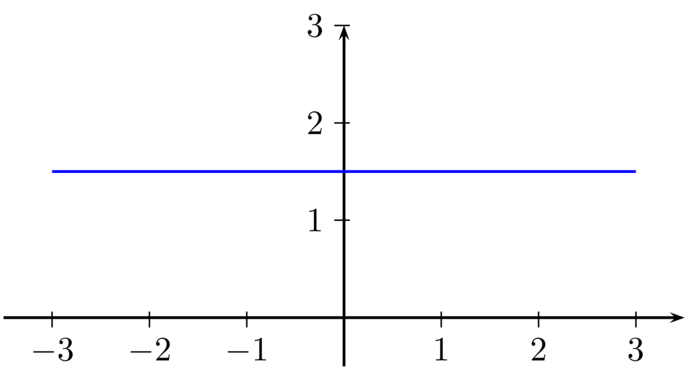
\includegraphics{Picture_FIGLabelFigFoncConstFdDkhWPICTFoncConstFdDkhW-for_eps.pdf}
%The result is on figure \ref{LabelFigFoncConstFdDkhW}.
%\newcommand{\CaptionFigFoncConstFdDkhW}{<+Type your caption here+>}
\input{Fig_FoncConstFdDkhW.pstricks}

\end{multicols}


\subsection{Sens de variation d'une fonction affine}

\begin{Aretenir}
      Soit $f$ la fonction affine $x\mapsto ax+b$.
      \begin{itemize}
      \item Si $a>0$, alors $f$ est croissante sur $\eR$.
      \item Si $a<0$, alors $f$ est décroissante sur $\eR$.
      \item Si $a=0$, alors $f$ est constante sur $\eR$
        (et $f(x)=b$ pour tout $x\in\eR$).
      \end{itemize}
\end{Aretenir}
Nous savons que si \( f(x)=ax+b\), alors \( f\) s'annule en \( x=-\frac{ b }{ a }\). Cela nous sert à écrire un tableau de signe de \( f\).



Les figures \ref{LabelFigFnAffineipcEQfssLabelSubFigFnAffineipcEQf0} et \ref{LabelFigFnAffineipcEQfssLabelSubFigFnAffineipcEQf1} montrent des droites affines. Lorsque \( a>0\), la droite monte; lorsque \( a<0\) elle descend. La pente est d'autant plus forte que \( a\) est grand.
\newcommand{\CaptionFigFnAffineipcEQf}{Deux droites affines.}
\input{Fig_FnAffineipcEQf.pstricks}


\begin{Aretenir}
      Règle du signe de $ax+b$ \\
      
      \begin{tabular}{cc}
        $a<0$ & $a>0$ \\
        & \\
        $\begin{array}{|c|ccccc|}
          \hline
          x & -\infty & & -\dfrac{b}{a} & & +\infty \\[2ex]
          \hline
          ax+b & & + \quad \ & 0 & \quad - & \\[1ex]
          \hline
        \end{array}$
        &
        $\begin{array}{|c|ccccc|}
          \hline
          x & -\infty & & -\dfrac{b}{a} & & +\infty \\[2ex]
          \hline
          ax+b & & - \quad \ & 0 & \quad + & \\[1ex]
          \hline
        \end{array}$ \\
      \end{tabular}  \\[1ex] 
\end{Aretenir}

\subsection{Tableau de variations}


Le \defe{tableau de variation}{tableau de variation} est un tableau contenant
\begin{enumerate}
    \item
        les positions des sommets,
    \item
        les flèches indiquant les endroits où la fonction est croissante ou décroissante.
\end{enumerate}
Un petit exemple valant mieux qu'un long discours\ldots

% à noter le 9 dans l'environnement suivant est le nombre de lignes sur lesquelles la figure s'étale. Je suis obligé de donner à la main parce que le tableau ne compte apparemment que pour une seule ligne. Du coup si je laisse à LaTeX le soin de calculer, les lignes de texte en-dessous de la figure (et en particulier à la page suivante si la figure est en bas de page) sont encore coupées.
\begin{wrapfigure}[9]{r}{6.0cm}     
   \vspace{-1cm}        % à adapter.
   \centering
   \input{Fig_GrapheVarREGMqx.pstricks}
\end{wrapfigure}

    Le tableau de variation de la fonction dessinée ci-contre est :
    \begin{equation*}
    \begin{array}[h]{|c|ccccccc|}
        \hline
        x&-3&&-2&&0&&2\\
        \hline
        &&&2&&&&1\\
        f(x)&&\nearrow&&\searrow&&\nearrow&\\
        &-\frac{ 9 }{2}&&&&-\frac{ 1 }{2}&&\\
        \hline
    \end{array}
    \end{equation*}
    En effet, la fonction \( f\)
    \begin{itemize}
        \item 
            part de \( x=-3\) où \( f(x)=-9/2\);
        \item
            elle monte jusqu'en \( x=-2\) où elle vaut \( f(x)=2\);
        \item
            elle descend jusqu'en \( x=0\) où elle vaut \( -\frac{ 1 }{2}\);
        \item
            elle monte jusqu'en \( x=2\) où elle vaut \( 1\).
    \end{itemize}

Le plus souvent si on donne un dessin, les nombres à placer dans un tableau de variation sont des valeur approchées à la précision du dessin. Donner les réponses en fraction n'est donc pas obligatoire. Par exemple ici au lieu d'écrire \( -9/2\) dans le tableau, il aurait été possible d'écrire \( -4.5\).

\section{Minimum et maximum}

Les notions de minima et maxima parlent, comme l'indiquent leurs noms en français, des points du graphe d'une fonction les plus hauts et les plus bas.

\begin{definition}
      Soit $f$ une fonction définie sur un intervalle $I$.
      \begin{itemize}
          \item On dit que $f$ admet le réel $m$ pour \defe{minimum}{minimum (d'une fonction)} sur $I$ si et seulement si il existe $c\in I$ tel que $f(c)=m$ et pour tout $x\in I$, $f(x)\geq m$. 
    \item On dit que $f$ admet le réel $M$ pour \defe{maximum}{maximum} sur $I$ si et seulement si il existe $d\in I$ tel que $f(d)=M$ et pour tout $x\in I$, $f(x)\leq M$.
      \end{itemize}
\end{definition}

Sur la figure \ref{LabelFigMinMaxKNRdOd}, nous avons indiqué le minimum et le maximum de la fonction dessinée.
\newcommand{\CaptionFigMinMaxKNRdOd}{Minimum et maximum d'une fonction.}
\input{Fig_MinMaxKNRdOd.pstricks}


%+++++++++++++++++++++++++++++++++++++++++++++++++++++++++++++++++++++++++++++++++++++++++++++++++++++++++++++++++++++++++++ 
\section{Exercices : généralités sur les fonctions}
%+++++++++++++++++++++++++++++++++++++++++++++++++++++++++++++++++++++++++++++++++++++++++++++++++++++++++++++++++++++++++++

%---------------------------------------------------------------------------------------------------------------------------
\subsection{Image, antécédent}
%---------------------------------------------------------------------------------------------------------------------------

\Exo{Seconde-0042}
\Exo{Seconde-0048}
\Exo{Seconde-0054}
\Exo{Seconde-0051}
\Exo{Seconde-0050}

%---------------------------------------------------------------------------------------------------------------------------
\subsection{Exemples de fonctions}
%---------------------------------------------------------------------------------------------------------------------------

\Exo{Seconde-0058}
\Exo{Seconde-0057}
\Exo{Seconde-0063}
\Exo{Seconde-0061}
\Exo{Seconde-0067}
\Exo{smath-0295}

%---------------------------------------------------------------------------------------------------------------------------
\subsection{Représentation graphique}
%---------------------------------------------------------------------------------------------------------------------------

\Exo{Seconde-0043}
\Exo{Seconde-0059}
\Exo{Seconde-0047}
\Exo{Seconde-0060}
\Exo{Seconde-0049}

\Exo{smath-0127}
\Exo{smath-0439}

%---------------------------------------------------------------------------------------------------------------------------
\subsection{Travail sur les graphiques}
%---------------------------------------------------------------------------------------------------------------------------

\Exo{Seconde-0069}
\Exo{Seconde-0070}
\Exo{Seconde-0071}

% TODO : ce serait pas mal de mettre une question pleine de texte ici.

\Exo{smath-0015}
\Exo{Seconde-0072}
\Exo{smath-0209}
\Exo{smath-0298}

%---------------------------------------------------------------------------------------------------------------------------
\subsection{Problèmes et résolution d'équation}
%---------------------------------------------------------------------------------------------------------------------------


\Exo{smath-0210}
\Exo{smath-0001}
\Exo{smath-0004}
\Exo{smath-0005}
\Exo{smath-0006}
\Exo{Seconde-0046}

\Exo{smath-0186}    % Cet exercice est le même que le smath-0111, mais vu différemment.
\Exo{smath-0078}
\Exo{smath-0013}
\Exo{Seconde-0068}
\Exo{Seconde-0064}
\Exo{Seconde-0044}
\Exo{Seconde-0066}
\Exo{Seconde-0075}
\Exo{Seconde-0076}

%---------------------------------------------------------------------------------------------------------------------------
\subsection{Plus avancés}
%---------------------------------------------------------------------------------------------------------------------------

\Exo{Premiere-0018}
